\chapter{Metodologia}\label{cap-metodologia}

% Descrever a metodologia dos testes, como variou o tamanho dos arquivos, quantos arquivos foram utilizados, descrição do computador em que foram feitos os testes.

Utilizando scripts de bash, pudemos automatizar os processos de testes, facilitando muito o levantamento de dados, possibilitando a obtenção de um maior espaço amostral e reduzindo os erros humanos. 

% 20?
Os testes foram realizados executando 20 iterações de um mesmo programa. Por exemplo, um carregamento de 10 arquivos com 500 buscas aleatórias seria repetido 20 vezes. Assim, garantimos que o espaço amostral seja satisfatório para a obtenção de dados pouco enviesados por \textit{outliers} --- neste caso, buscas e inserções muito lentas ou muito rápidas --- sobre a execução do programa.

Além disso, todos os testes foram efetuados em duas máquinas diferentes. A Máquina 1 possui 8GB de RAM e um processador AMD FX-6300 com 6 núcleos rodando a 3.80GHz com um sistema operacional Linux Mint 19.1; já a Máquina 2 conta com 16GB de RAM e um processador Intel i7-7XXX com 8 núcleos rodando a XGHz e um sistema operacional Linux Ubuntu X.

Os arquivos utilizados para testes variaram de 1KB a cerca de 10MB, de 1 a 15 arquivos por vez. Arquivos com mais de 20MB usualmente demoram mais de uma hora para carregar em todas as estruturas, portanto este foi o limite estipulado pelos nossos testes.

\section{Resultados}

Analisar os tamanhos dos arquivos compactados a partir dos experimentos realizados. Utilizar tabelas e gráficos para ilustrar o desempenho da sua implementação.








\begin{comment}

Exemplo de utilização de tabelas.  A Tabela ~\ref{tab:cronograma-1} apresenta um cronograma de execução de um PG fictício.

\begin{table}[htb]
	\centering
	\caption{Cronograma de Atividades do primeiro semestre.}
	\label{tab:cronograma-1}
	\resizebox{\columnwidth}{!}{
		\begin{tabular}{c|c|c|c|c|c|c}
			Atividade & Janeiro/99 & Fevereiro/99  & Março/99  & Abril/99 & Maio/99 & Junho/99\\ \hline
			1&     X      &  	  X   	       &  	X	  	   & 		X	&     X   &      X    \\ \hline
			2&            &  	   	     	   &  	  X  	   & 		X	&         &           \\ \hline
			3&            &  		           &  	  X 	   & 		X   &   X     &     X      \\ \hline
			4&            &  			       &  			   & 	        &         &     X      \\ \hline
			5&            &  			       &  			   & 	        &    X    &   X       \\ \hline
			6&            &  			       &  			   & 	        &         &           \\ \hline
			7&            &  			       &  			   & 	        &         &           \\ \hline
		\end{tabular}
	}
\end{table}

A Figura \ref{fig:graf} exemplifica o uso de uma figura gráfica no texto.

\begin{figure}[!htb]
\centering
%   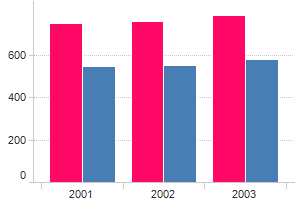
\includegraphics[scale=0.90]{figuras/graf-exemplo.png}
  \caption{Exemplo de inserção de figura}
  \label{fig:graf}
\end{figure}
\end{comment}
